\documentclass[spanish]{amsart}
\usepackage{babel}
\usepackage[margin=0.8in]{geometry}
\usepackage[utf8]{inputenc}
\usepackage{graphicx}
\usepackage{babel}
\usepackage{hyperref}
\usepackage{amsrefs} % use [alphabetic] for author name citations.
\usepackage{upgreek}
\usepackage{physics}
\usepackage{color, soul}

\newtheorem{lemma}{Lema}
\newtheorem{corollary}{Corolario}
\newtheorem{proposition}{Proposición}
\newtheorem{theorem}{Teorema}

\makeatletter


\title{Descripción de la geometría del espacio de móduli del funcional
  de Ginzburg-Landau}

\author{Ren\'e Garc\'{\i}a}
\address{School of Mathematics\\University of Leeds\\Leeds, UK}

\newtheorem*{assertion}{Assertion}
\newtheorem*{definition}{Definición}
\newtheorem*{remark}{Remark}


\newcommand{\delbar}{\bar{\partial}_A}
\newcommand*{\R}{\mathbb{R}}
\newcommand*{\C}{\mathbb{C}}
\newcommand*{\hatC}{\widehat{\mathbb{C}}}
\newcommand*{\del}{\partial}
\newcommand*{\delz}{\del_z}
\newcommand*{\delzbar}{\del_{\bar{z}}}
\newcommand*{\cpone}{\mathbb{P}^1}
\newcommand*{\metric}{\mathfrak{h}}
\newcommand*{\moduli}{\mathcal{M}}
\newcommand*{\kahler}{K\"ahler{ }}
\newcommand*{\bog}{Bogomol'nyi{ }}
\newcommand*{\bogs}{Bogomol'nyi's{ }}
%\newcommand*{\moduli}[1][n_+,n_-]{M^{#1}}
\newcommand*{\lagrangian}{\mathcal{L}}

\DeclareMathOperator{\energy}{E}
\DeclareMathOperator{\J}{J}


\begin{document}
\maketitle
\begin{abstract}
  Un problema clásico de física-matemática es la descripción del
  espacio de vórtices del funcional de Ginzburg-Landau. Se le llama de
  esta manera a las soluciones de mínima energía del problema
  variacional estudiado por Ginzburg y Landau para modelar propiedades
  superconductoras de la materia. Las soluciones extremas del
  funcional forman un espacio de dimensión infinita, pero módulo
  equivalencia de norma, existe una subvariedad Riemanniana de
  dimensión finita cuya descripción geométrica se relaciona con las
  propiedades físicas de los superconductores.
\end{abstract}


\section{Dinámica de solitones}
\label{sec:soliton-dynamics}

Los solitones son regiones localizadas de energía de un campo, puede
ser escalar o vectorial. Varios sistemas de ecuaciones diferenciales
de interés en física matemática poseen soluciones solitónicas o
aproximaciones de este tipo. Por
ejemplo, al modelar el vuelo de un avión que rompe la barrera del
sonido, o la estructura del núcleo atómico a bajas energías
\cite{manton2004topological}. Una conjetura de Nick Manton dice que la
dinámica de solitones lentos en varias teorías físicas
(Yang-Mills-Higgs, Campo de Higgs abeliano y modelo \(\sigma \) no
lineal), se pueden aproximar con el movimiento geodésico en el espacio
de móduli correspondiente \cite{manton198254}. 

Entonces, el estudio de la geometría riemanniana del espacio de móduli
de solitones se utiliza para entender la dinámica de solitones
lentos \cite{samols1992}.
 
\section{El lagrangiano de Ginzburg-Landau}
\label{sec:GL-lagrangiano}

El modelo abeliano de Higgs \cite{PhysRev.145.1156} es un modelo
simple exhibiendo el mecanismo de Higgs. Este modelo exhibe soluciones
estables llamadas vórtices, y una simplificación asumiendo simetría
traslacional reduce el problema a \(1 + 2 \) dimensiones de
espacio-tiempo \cite{samols1992}. Sea \(\psi: \psi_1 + \psi_2i: \R\times\C \to
\C\) un campo escalar dependiente del tiempo. El campo de Higgs, y
\(A_{\mu} \) una forma de conexión del haz de línea complejo,
necesariamente trivial,
sobre el espacio-tiempo, \(\R\times\C \). La densidad lagrangiana del
campo, acoplado con el campo de norma, es

\begin{equation}
\label{eq:GL-lagrangian}
\lagrangian = \frac{1}{2} D_{\mu}\psi\overline{D^{\mu}\psi} -
\frac{1}{4}F_{\mu\nu}F^{\mu\nu} - \frac{1}{8}\lambda (\abs{\psi}^2 - 1)^2,
\end{equation}

donde \(D_{\mu}\psi = \del_{\mu}\psi - iA_{\mu}\psi \), es la derivada
covariante del campo, y \(F_{\mu\nu} = \del_{\mu}A_{\nu} -
\del_{\nu}A_{\mu} \) es la curvatura de la forma de conexión. En la
teoría de superconductividad de Ginzburg-Landau, la constante positiva
\(\lambda \) determina el tipo de superconductor. Si \(\lambda < 1 \),
la superficie superconductora que representa el dominio espacial del
campo de Higgs es del tipo I, o si \(\lambda > 1 \) es del tipo II. La
signatura del espacio tiempo es \((+1, -1, -1) \), y si separamos la
densidad lagrangiana según los factores temporales, resulta la
descomposición en energía cinética y potencial del sistema
\cite{manton2004topological}

\[
L = T - V,
\]

donde

\begin{equation}
\label{eq:kinectic-energy}
T = \frac{1}{2}\int_{\C} \abs{D_0\psi}^2 - \abs{E}^2 dx, \qquad
V = \frac{1}{2}\int_{\C} D_j\psi\overline{D^j\psi} + \abs{B}^2 +
\frac{1}{8}\lambda(\abs{\psi}^2- 1)^2dx,
\end{equation}

\(E = F_{0k}\,dt\wedge dx^k \) es la forma de campo eléctrico y \(B =
F_{jk}dx^j\wedge dx^k\) es la forma de campo magnético
\cite{frankel_2011}. El principio
variacional \cite{giaquinta2004calculus} dice que la pareja \((\psi,
A) \) que corresponda a un
campo físicamente relevante, debe de ser un extremal del funcional de
acción,
\[
S[\psi, A] = \int_{\R}L dt.
\]
Aplicando el principio variacional, una pareja \((\psi, A) \) que deje
invariante la acción a primer orden, debe de satisfacer las ecuaciones
de Euler Lagrange:
\begin{equation}
  \label{eq:euler-lagrange-equation}
  \begin{split}
      D_{\mu}D^{\mu}\psi + \frac{1}{2}\lambda\psi(\abs{\psi}^2 - 1) &= 0,\\
  \del_{\mu}F^{\mu\nu} + \Im{\psi\,\overline{D^{\nu}\psi}} &= 0.
  \end{split}
\end{equation}
(\ref{eq:euler-lagrange-equation}) es un sistema acoplado de
ecuaciones diferenciales parciales que no se puede resolver de manera
analítica.

Nótese que el grupo unitario \(U(1) \) actúa por isometrías en el haz
de líneas complejo del cuál \(\psi \) es una sección, y que la
densidad lagrangiana es invariante bajo al acción del grupo, la cuál
es
\begin{equation}
\label{eq:u1-action}
\begin{split}
  \psi &\mapsto e^{i\alpha(x)}\psi,\\
  A_{\mu} &\mapsto A_{\mu} + \del_{\mu}\alpha,
\end{split}
\end{equation}
donde \(U(1) \) actúa fibra a fibra con la representación
\(e^{i\alpha(x)}\).

\begin{definition}
  El espacio de móduli de vórtices  \(\moduli \) es el espacio
  cociente del espacio de soluciones del problema variacional, \((\psi,
  A) \), con energía finita, módulo la acción del grupo de norma
  (\ref{eq:u1-action}).
\end{definition}

La energía total del vórtice es
\[
E = \int_{\R}T + V dt,
\]
y la condición de finitud de la energía restringe la forma de \((\psi,
A) \) en el infinito. \((\psi, A )\) es un campo vacío si es norma
equivalente a \( \psi \equiv 1\), \(A \equiv 0 \). Para que la energía
sea finita, \((\psi, A) \) se debe de aproximar, salvo transformación
de norma, a un campo vacío, cuando \(z \to \infty \), \(z \) la
variable espacial del dominio.

Una vez dadas las definiciones básicas de teoría de campos, nuestro objetivo es describir el espacio de móduli. Una conjetura de
Nick Manton dice que describir el espacio de vórtices que se
mueven lentamente se puede hacer, considerando primero el espacio de
vórtices estáticos, y suponiendo que el movimiento de vórtices lentos
se puede aproximar en el moduli estático \cite{manton198254}. Esta
idea de Manton ha sido probada por Stuart en dos y tres dimensiones
espaciales \cite{stuart1994geodesic}, \cite{stuart1994dynamics}. Para
vórtices estáticos, lo que se minimiza es la energía potencial \(V \)
dada en la ecuación (\ref{eq:kinectic-energy}), y las ecuaciones
resultantes en dos dimensiones espaciales son
\begin{equation}
  \label{eq:static-euler-lagrange}  
  \begin{split}
    D_jD^j\psi + \frac{1}{2}\lambda\,\psi(\abs{\psi}^2 - 1) &= 0,\\
    \epsilon_{jk}\del_jF^{12} + \Im{\psi\,\overline{D^{k}\psi}} &= 0.
  \end{split}
\end{equation}

Como \(F^{12} \) es la única componente del campo magnético
perpendicular a la superficie del plano complejo, si definimos \(J^k = -
\Im{\psi\,\overline{D^{k}\psi}}\), entonces la segunda ecuación es una
versión bidimensional de la ley de Ampere, \(\nabla\times b = J \).


\section{Solitones topológicos}
\label{sec:topological-solitons}

A partir de ahora, supondremos que la constante de acoplamiento tiene
el valor crítico \(\lambda = 1 \). Supongamos que existe una función
suave \(\chi:S^1 \to \R \), tal que, si \(z = re^{i\theta} \),
entonces \(\psi \) se aproxima asintóticamente a \(e^{i\chi(\theta)} \)
mientras \(r\to\infty \). La condición de energía finita también
implica que
\[
D_{\theta}\psi = \del_{\theta}\chi - A_{\theta} = 0.
\]
Como corolario,
\begin{equation}
\label{eq:vortex-number}
2\pi\int_{\C} F_{12}dx = 2\pi\int_0^{2\pi}A_{\theta} = 2\pi N.
\end{equation}
El número \(N \) es el \emph{número de vórtice}, y es un invariante
topológico, tal que el espacio de móduli, es un espacio estratificado,
según este número. \(N \) también se puede interpretar, suponiendo que
\(\psi \) tiene una cantidad finita de ceros de multiplicidad 1, de
manera que el número de vórtice mide cuando ceros, tomando en cuenta
la orientación, tiene el campo.

\begin{definition}
  Si \(z_0 \) es un cero simple de \(\psi \), tal que 
  el número de vuelta alrededor de la frontera de una
  \(\epsilon \) vecindad suficientemente pequeña, es positivo, se dice
  que \(z_0 \) es la posición de un vórtice. En caso contrario, si el
  número de vuelta es negativo, se dice que \(z_0 \) es la posición de
  un antivórtice.
\end{definition}

A continuación, considera el caso de un vórtice estático. La energía
total del vórtice, es la energía potnecial \(V \), la cuál puede ser
reescrita con la integral siguiente:
\begin{equation}
  \label{eq:potential-energy}
\begin{split}
  V &= \frac{1}{2} \int_{\C}(D_1 \pm iD_2)\psi\;\overline{(D_1 \pm
    iD_2)\psi} + \left( F_{12} \pm \frac{1}{2}(\abs{\psi}^2 - 1)
  \right)^2 \\
  &+ i \left( \del_2(\bar{\psi}D_1\psi) -
    \del_1(\bar{\psi}D_2\psi) \right) \pm F_{12} \,dx.
\end{split}
\end{equation}

La expresión anterior se conoce como el truco de \bog
\cite{Bogomolny}. Nótese que es 
esencial que el valor de la constante es el valor crítico, \(\lambda =
1\). 

\begin{proposition}[Cota de Bradlow]
  Para vórtices estáticos de energía \(E \), el número de vórtice
  satisface la cota
  \[
E \geq \pi \abs{N}.
  \]
\end{proposition}

\begin{proposition}[Ecuaciones de \bog]
  Si \((\psi, A) \) es una solución estática de mínima energía,
  entonces,
  
\begin{equation}
  \label{eq:bog-equations}  
\begin{split}
D_1\psi \pm iD_2\psi &= 0,\\
F_{12} \pm \frac{1}{2}(\abs{\psi}^2 - 1) &= 0.
\end{split}
\end{equation}
\end{proposition}

\begin{proof}
Ambas proposiciones son consecuencia de la ecuación (\ref{eq:potential-energy}).
\end{proof}

La ventaja que tienen las ecuaciones de \bog sobre el principio
variacional es que son de un orden menor. Nótese que
(\ref{eq:bog-equations}) sólo es válido para vórtices estáticos. 

\section{La solución de Taubes}
\label{sec:taubes-equation}

Sea \(\hat{A} = A_1 + A_2\,i \), entonces las primeras ecuaciones de
\bog son equivalentes a
\begin{equation}
\label{eq:bog-complex}
2\delzbar \psi - i\hat{A}\psi = 0,
\end{equation}
de aquí, se puede escribir formalmente \(\hat{A} =
-2i\delzbar\ln(\psi) \). Supongamos que existe una función compleja
\(f = f_1 + f_2i \), tal que \(\psi = e^f \) fuera de los ceros de
\(\psi \). La condición que \(\abs{\psi} \to 1 \) en el infinito, es
equivalente a requerir que \(\lim_{z\to\infty}f_1 = 0 \).  Más aún, \(f_1 \) debe de
satisfacer la ecuación
\begin{equation}
\label{eq:taubes}
-\laplacian f_1 + \frac{1}{2} (e^{2f_1} - 1) = 0.
\end{equation}
fuera de los zeros de \(\psi \). La ecuación (\ref{eq:taubes}) es la
ecuación de Taubes. Una suposición común es que los vórtices se
encuentran separados, de manera que los ceros de \(\psi \) son
simples. Un argumento asintótico a los ceros de \(\psi \) demuestra
que si este es el caso, entonces las singularidades de \(f_1 \) deben
de ser de tipo la función \(\delta \) \cite{taubes1980}, de modo que
la ecuación de Taubes, extendida a todo el plano complejo, es
\begin{equation}
  \label{eq:taubes-extended}
-\laplacian f_1 + \frac{1}{2} (e^{2f_1} - 1) = \sum_n\delta(z - z_n),
\end{equation}
junto con la condición de frontera en el infinito que \(f_1 \to 0
\). Si existe una solución de (\ref{eq:taubes-extended}), entonces las
ecuaciones (\ref{eq:bog-equations}), (\ref{eq:bog-complex}) permiten
recuperar  \(\psi \) y \(A \), porque de ellas se deduce que 
\begin{align}
  A_1 &= \del_2f_1 + \del_1f_2,\\
  A_2 &= -\del_1f_1 + \del_2f_2,\\
  F_{12} &= - \laplacian f_1.
\end{align}
Estas ecuaciones, junto con la topología de \(\C \) que es simplemente
conexo, permiten inferir \(A \) a partir de \(F \), y posteriormente
\(f_2 \), módulo un término de la forma \(2\pi\,n \), que tiene que
ver con la libertad de norma. 

\begin{theorem}
  [Taubes, 1980]
  Para cada conjunto de puntos en el plano \((a_1,\ldots, a_n) \),
  existe una única solución \(C^{\infty} \) de la ecuación
  (\ref{eq:taubes-extended}) con las condiciones de frontera al
  infinito correspondientes, tal que \((a_1,\ldots, a_n) \) es el
  conjunto de ceros de \(\psi \).
\end{theorem}

En el mismo artículo \cite{taubes1980}, Taubes demuestra que el
conjunto de ceros de cualquier campo de Higgs estático es discreto.

\section{Fórmula de localización de Samols}
\label{sec:samols-localization-formula}

Si consideramos el tiempo como un parámetro extra, en lugar de una
coordenada más en el espacio de configuración, entonces la energía
cinética funciona como una métrica en el espacio de móduli. Esta idea
es de Manton \cite{manton198254} y para vórtices fue hecha rigurosa
por Stuart \cite{stuart1994dynamics}. La idea se resume en la
siguiente figura, tomada de la referencia estándard
\cite{manton2004topological}.

\begin{center}
  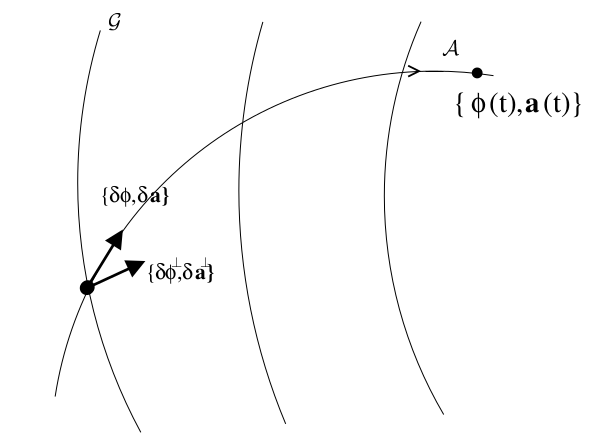
\includegraphics[width=0.3\linewidth]{img/mantons-idea}
\end{center}

Consideremos la norma de radiación, \(A_0 = 0 \), de modo que
\(D_0\psi = \dot{\psi}\), y \(F_{0j} = \dot{A_j} \). La energía
potencial es un invariante de norma. Lo que nos gustaría saber es,
dada una órbita, cómo calcular un invariante de la órbita, que no
dependa del levantamiento, sino de la proyección al espacio de móduli
\(\moduli \). Entre el tiempo \(t \) y \(t + \delta t \), la
contribución a la energía cinética de cualquier trayectoria \((\psi(t),
A_j(t)) \) es
\begin{equation}
  \label{eq:moduli-kinectic-energy}
\frac{1}{2} \frac{1}{(\delta t)^2}\int_{\C} \left( \delta a \cdot
  \delta a + \overline{\delta \psi}\,\delta\psi \right) dx,
\end{equation}
donde \(\psi \mapsto \psi + \delta\psi \), \(A_j \mapsto A_j + \delta
A_j \), son las variaciones de los campos. La ecuación
(\ref{eq:moduli-kinectic-energy}) no es invariante bajo la acción del
grupo de norma, pero si \(\alpha: \C \to \R \) es un campo en el
álgebra de Lie trivial de \(U(1) \), y definimos
\begin{equation}
  \label{eq:beta-variation}
  \begin{split}
  \delta'\psi &= \delta \psi - i\alpha\psi, \\
  \delta' A &= \delta A - \nabla \alpha,    
  \end{split}
\end{equation}
entonces el funcional
\begin{equation}
\label{eq:moduli-invariant-kinectic-energy}
\Pi[\alpha] = \frac{1}{2} \int_{\C} \left( \delta' A \cdot \nabla\alpha +
  \frac{1}{2} \left( \delta'\psi \overline{(i\alpha\psi)} +
    \overline{\delta'\psi}\, i\alpha\psi\right) \right) dx,
\end{equation}
sí será invariante. Suponiendo que exste un campo \(\beta \), tal que
\(\Pi[\beta] = 0 \) y aplicando integración por partes, \(\beta \)
debe de satisfacer la ecuación

\[
(\laplacian - \abs{\psi}^2)\beta = \nabla\cdot \delta A -
\Im{\bar{\psi}\delta \psi}.
\]

Refiriéndonos nuevamente a la ecuación (\ref{eq:beta-variation}), para
el campo \(\beta \), y haciendo la identificación \(\delta A =
\dot{\psi} \), \(\delta A_j = \dot{A}_j \), la interpretación es que
para una trayectoria \((\psi, A) \) en el espacio de móduli, la
variación con este campo \(\beta \) corresponde a la proyección
ortogonal en la configuración inicial.

\begin{proposition}
  [Manton, 1982] Sean \(\psi^{\perp} \), \(A^{\perp} \), las variaciones
  correspondientes al campo \(\beta \), entonces, si suponemos que la
  ley de Gauss se cumple,
  
\begin{equation}
\label{eq:energy-variation-correspondence}
\frac{1}{2} \int_{\C}e_ie^i + \overline{D_0\psi}\,D_0\psi dx =
\frac{1}{2} \int_{\C}\dot{A}_j^{\perp}\dot{A}^{j\perp} +
\overline{\del_0\psi^{\perp}}\,\del_0\psi^{\perp} dx.
\end{equation}
\end{proposition}

Por lo tanto, la energía cinética del campo se puede ver como un
invariante de norma que corresponde a la proyección ortogonal de la
trayectoria en el tiempo del par \((\psi, A) \). Si pensamos en \(t \)
como un parámetro, siendo muy imprecisos en las definiciones, la
energía cinética define el equivalente a la norma \(L_2 \) en el
espacio tangente a las trayectorias que físicamente corresponden con
la realidad.

Consideremos a continuación el móduli de soluciones estáticas,
entonces el teorema de Taubes garantiza que este móduli puede ser
identificado con un espacio discreto, pues las soluciones son
dependientes de las posiciones de los ceros, que son discretas, así
que el espacio de móduli estático también es un espacio estratificado,
en el cuál cada estrato corresponde con el número de vórtice:

\begin{equation}
\label{eq:moduli-decomposition}
\moduli_{stat} = \cdots \moduli_{stat}^{-1} \sqcup \moduli_{stat}^0
\sqcup \moduli_{stat}^{1} \cdots
\end{equation}

A su vez, cada estrato es otra unión de copias de \(\C \), de la forma
\(\C^{n_1} \times \C^{n_2} / \sim \), donde \(n_1, n_2\in\mathbb{Z} \) es
el número de vórtices y antivortices respectivamente, tales que \(n_1
+ n_2 = n \) es el número de vórtice. y la relación de equivalencia
que corresponde al grupo simétrico, esporque dos vórtices o dos
antivórtices son indistingibles. Es un problema abierto describir la
topología de los espacios de móduli, sin embargo, Samols describió
como calcular la energía cinética fuera de la región de Coalescencia
para un par \(\psi(\cdot, z_1, \cdots z_n), A(\cdot, z_1, \cdots, z_n)
\), suponiendo que la variación en el tiempo es representada por la
variación de las posiciones de los ceros \cite{samols1992}.


\begin{theorem}
  [Samols, 1992] Sea \(b_s = 2\,\delz\left( f_1 - \ln\abs{z - z_s}^2
  \right) \), entonces fuera de los puntos de coalescencia,
  \[
ds^2 = \frac{1}{2} \sum_{r,s}^n\left( \delta_{rs} + 2 \frac{\del
    \bar{b}_s}{\del z_r} \right) dz_rd\bar{z}_s,
\]
donde \(n \) es el número de vórtice. Más aún, la métrica es Kahler,
con la forma de Kahler
  \[
\omega = \frac{i}{4} \sum_{r,s}^n\left( \delta_{rs} + 2 \frac{\del
    \bar{b}_s}{\del z_r} \right) dz_r\wedge d\bar{z}_s,
\]
\end{theorem}

La fórmula de Samols nos da una manera de estudiar la geometría del
espacio de móduli, de manera tanto analítica como numérica. Sin
embargo no existe una expresión algebraica para los coeficientes \(b_s
\). Se puede deducir por ejemplo que en el espacio de móduli estático,
si las curvas geodésicas representaran partículas en un sistema
mecánico, estas conservarían el momento y momento angular, y tendrían
centro de masa
\begin{equation}
\label{eq:centre-of-mass}
Z = \frac{1}{n} \sum z_r.
\end{equation}
de modo que el móduli \(M_{stat}^n \) tiene una despomposición extra
\(\C \times M_0^n\), donde \(M_0^n \) corresponde a movimiento en el
centro de masa. En el mismo artículo, Samols resuelve el problem de un
par vórtice antivortice, y llega a la conclusión que la geometría en
el centro de masa es cónica, en el sentido descrito en la siguiente
imagen, tomada de \cite{samols1992}
\begin{center}
  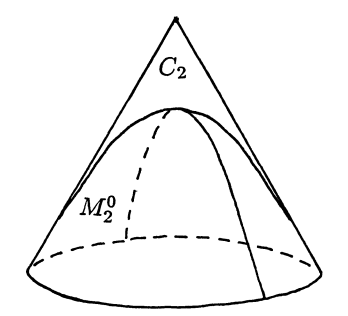
\includegraphics[width=0.3\linewidth]{img/conic-geometry}
\end{center}

Nótese que la geometría descrita por Samols es la geometría del
espacio de móduli estático. Sin embargo, Yang demuestra
\cite{yang1999strings} que la trayectoria real dependiente del tiempo
diverge de la trayectória estática exponencialmente, así que para un
intervalo de tiempo muy pequeño, la aproximación geodésica describe
las propiedades geométricas del espacio de móduli. Por ejemplo, la
siguiente gráfica del artículo de Samols muestra una simulación de la
dispersión de un par de vórtices
\begin{center}
  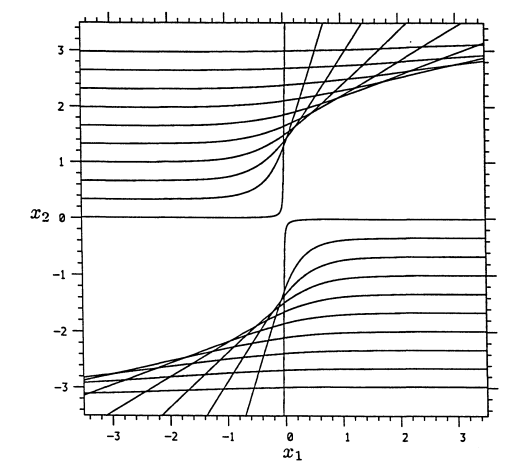
\includegraphics[width=0.3\linewidth]{img/vortex-scattering}
\end{center}

\bibliographystyle{plain}
\bibliography{refs}{}
\end{document}


%%% Local Variables:
%%% mode: latex
%%% TeX-master: t
%%% reftex-default-bibliography: ("refs.bib")
%%% TeX-source-correlate-method-active: synctex
%%% flyspell-default-dictionary: "spanish"
%%% ispell-local-dictionary: "spanish"
%%% coding: utf-8
%%% End:
